\chapter{Introduction}

\section{Background Information and Motivation}\label{background_information}

An alloy of iron and carbon: steel has notable durability with superior mechanical characteristics. Based on the evolving ability of its microstructures~\cite{bhadeshia2017steels, Tasan2015}, steel compositions can be obtained in a wide range, and they can be recycled without loss of property. Those make steel an excellent material to meet the ever-changing requirements of our contemporary society.

A modern steel manufacturing facility has a complex structure consisting of various production lines and can process a set of products successively. Fundamental steel manufacturing steps with respective production units are shown in Fig.~\ref{figure-steel-production-steps}~\cite{sinha-spinks_2015}. Raw materials are melted in the blast, electric arc or basic oxygen furnaces to obtain liquid iron. In the next step, liquid steel alloy is sent to the continuous casting line. It is poured into a mould cavity where it starts to cool. Right after, it is treated in a secondary cooling process with water sprays until it solidifies. A further production line involves a rolling process, which can be performed in two different modes: hot rolling and cold rolling. It allows obtaining the desired mechanical properties of steel, uniform thickness, a control on width dimension, and converting material to a flat and rectangular slab, a semi-finished steel product. The solid steel is heated in a reheat furnace before it's subjected to high pressures in the hot rolling unit. Before the cold rolling process, steel is treated with pickling to remove rust and impurities on the slab surface; it makes it easier to work on the material. The cold rolling unit improves surface finish and flatness, and it allows to modify metal work hardening. After the rolling process, slabs might be converted into compact coils featuring high lengths unless they will not be sent to further process units on the continuous production line, such as a galvanising line. It is the application of protective zinc coating on the steel surface to improve corrosion resistance.

The whole continuous production process is scheduled in a sequencing fashion, and production events are grouped into production batches (the so-called production sequences). Production sequences are arranged by the common properties of production orders and priority. Various constraints arise in technical, logistic, physical and chemical aspects~\cite{cowling2001design, OZGUR2021106606} due to different machines and production lines; having efficient sequence planning is necessary to cope.
\clearpage

 \begin{figure}[!ht]
	\begin{center}
		\makebox[\textwidth]{
			\centering
			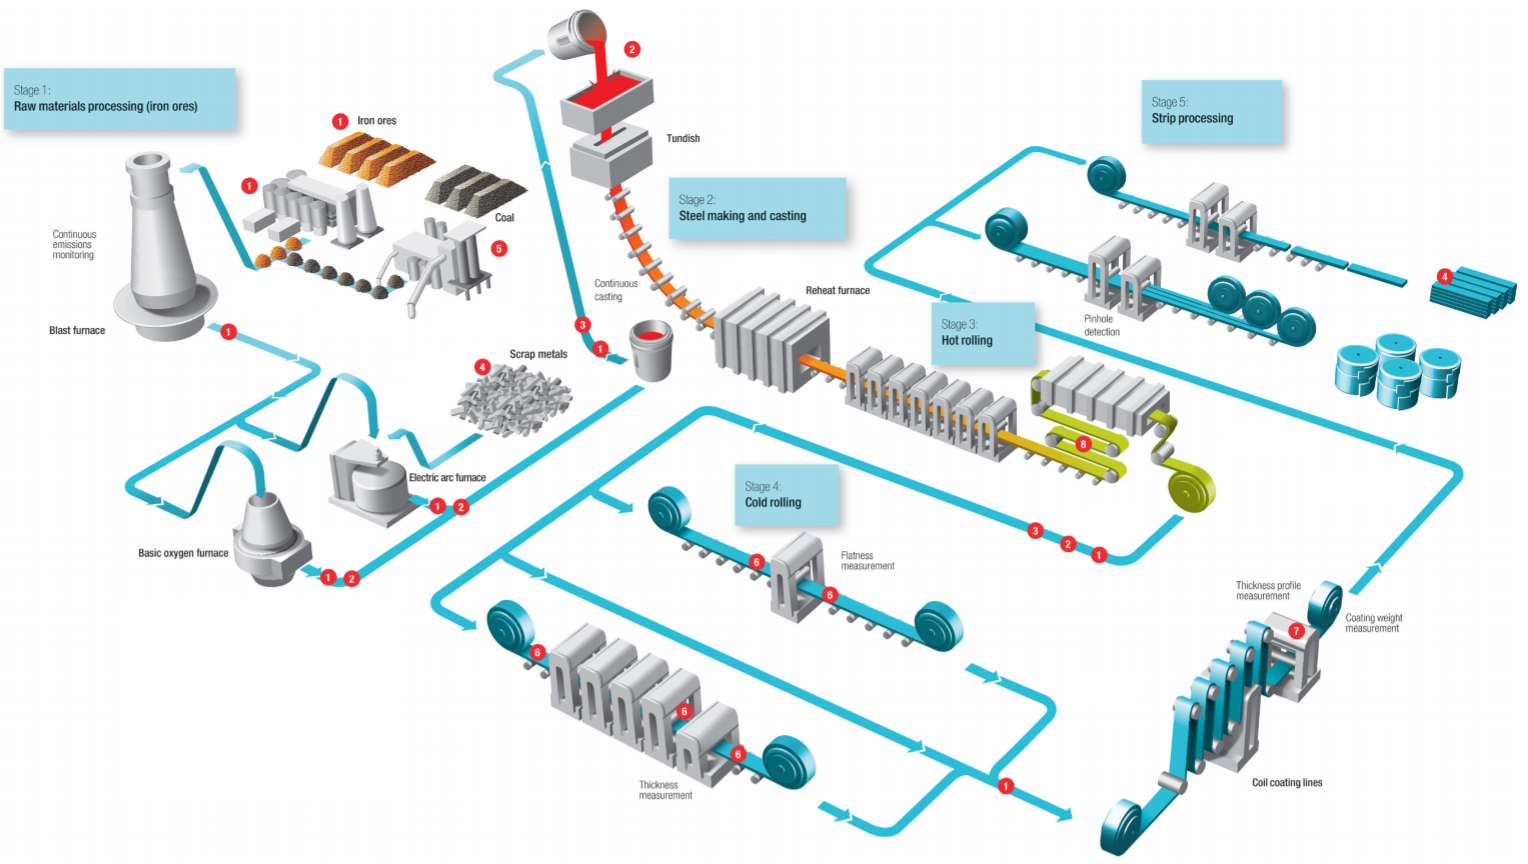
\includegraphics[width=1.0\linewidth]{../images/steel-production-steps.png}}
		\caption{Steel Manufacturing Steps~\cite{sinha-spinks_2015}.}
		\label{figure-steel-production-steps}
	\end{center}
\end{figure}

The above-explained processes and workstations can be arranged as a variety of integrated solutions based on the requirements of different demands or facility organisations. Table~\ref{Tab: production_lines} shows four production lines that the SMS group supplies~\cite{BRS}.
\begin{table}[ht!]
	\centering
	\setlength{\arrayrulewidth}{0.75pt}% 
	\caption{Compact Production Lines with Various Machine Modules.}
	\begin{tabular}{|c|c|c|}
		\hline
		\cellcolor[HTML]{FFFFC7} 
		No & \cellcolor[HTML]{FFFFC7} \begin{tabular}[c]{@{}c@{}}Production \\ Unit / Line\end{tabular} & \cellcolor[HTML]{FFFFC7} Description \\ \hline
		1               & \makecell{Continuous Casting\\Machine (CCM)}            & \makecell{Steel cools, passing through \\ the mould cavity and \\solidifies after water spraying.}  \\ \hline
		2               & \makecell{Compact Strip \\Production (CSP)}              &\makecell{Compact plant including CCM,\\   reheating furnace, hot rolling unit \\and strip processing unit.}       \\ \hline
		3               & \makecell{Pickling Line \& Tandem \\Cold Mill (PLTCM)} & \makecell{Compact plant including a\\   turbulence pickling section \\and a tandem mill.}                     \\ \hline
		4               & \makecell{Continuous Galvanizing \\Line   (CGL)}         & \makecell{Application of protective zinc \\  coating on the steel surface to \\improve corrosion resistance.} \\ \hline
	\end{tabular}
	\label{Tab: production_lines}
\end{table}

Steel manufacturing factory systems are automated with combined computer control and digital information. The sensory information received from production line machines concerning production orders (the so-called production events) is stored as data within a server to be incorporated with planning progress to provide functionality, adaptability and effective resource allocation in manufacturing processes~\cite{Saadaoui2019}. A data collection of production events from a steel manufacturer was pulled from the SMS group database to investigate. The queries in \ac{sql} were generated to find the production events across $2$--$3$ years of production work completed in the production lines, introduced in Table~\ref{Tab: production_lines}. The SQL queries are attached as supplementary materials, \ref{figure-supplements-CCM_CSP-SQL}, \ref{figure-supplements-PLTCM-SQL}, and \ref{figure-supplements-CGL-SQL}. The query attributes and resulting attribute values are anonymous. Further details for the data collection and cleaning steps are given in Subsection~\ref{data_collection_cleaning}.

After manipulation and cleaning steps were performed, CCM, CSP, PLTCM, and CGL data sets have the number of events, $347418$, $205496$, $59604$, and $27147$, respectively. The decreasing number of events through the data sets shows that the output of a production line is not always an input for the next in line and might be excluded from downstream production lines, as previously mentioned. As shown in Fig.~\ref{figure-thickness_diversity}, the number of events handled decreases with a slightly reduced width variety from CSP to CGL. Moreover, the production events in PLTCM and CGL have a wide diversity and precision in a narrow range for the thickness feature. In contrast, the events in CSP have a precise unimodal distribution gathered around a single value in a broad range of the same feature values.

 \begin{figure}[!ht]
	\begin{center}
		\makebox[\textwidth]{
			\centering
			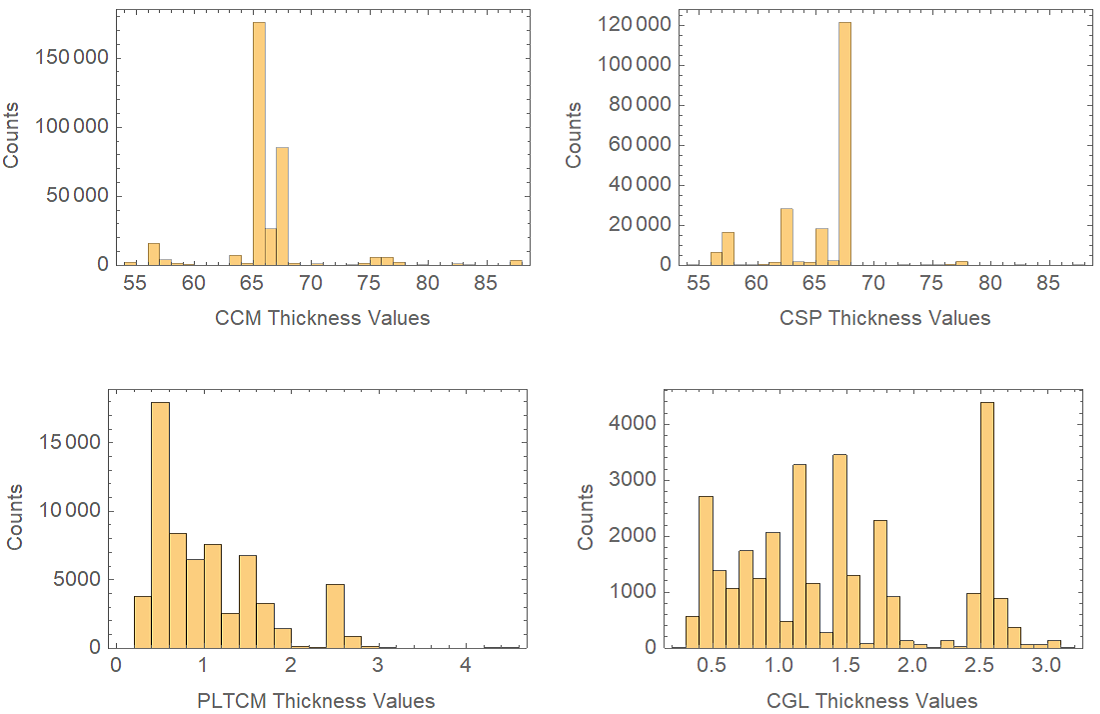
\includegraphics[width=1.05\linewidth]{../images/introduction-thickness_diversity.png}}
		\caption{Diversity in Event Features for Different Production Lines.}
		\label{figure-thickness_diversity}
	\end{center}
\end{figure}

Based on the summary of production data sets given above, the features of the production orders lose diversity and gain more precision as going further from CCM and CSP to PLTCM and CGL. In other words, a more generic production plan gives its place to a plan with more speciality among the production events.

 \begin{figure}[!ht]
	\begin{center}
		\makebox[\textwidth]{
			\centering
			\captionsetup{width=0.5\linewidth}
			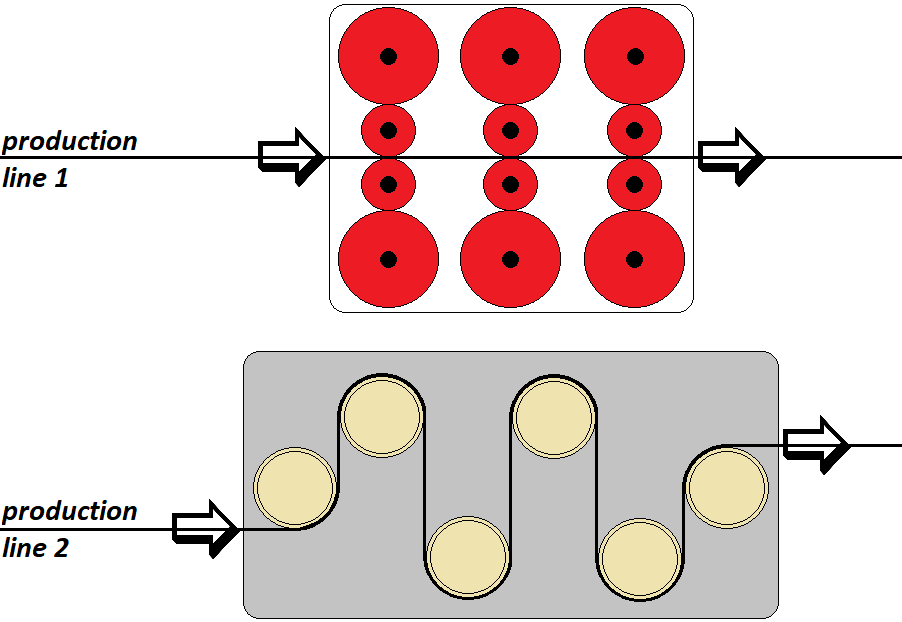
\includegraphics[width=0.9\linewidth]{../images/introduction-hypothetical_constraints.png}}
		\caption{Different Categories of Production Events Handling. The hot rolling mill positioned in production line 1 treats only one slab at a time. The unit in production line 2, pickling tank full of acid coloured in grey, treats the metal surface of more than one slab at a time.
		}
		\label{figure-hypothetical_constraints}
	\end{center}
\end{figure}

In addition to the diversity of the products, one can also see the handling operation differs between those production lines. Fig.~\ref{figure-hypothetical_constraints} illustrates alternative handling categories for the production events in two separate production lines. The machine in production line 1 can handle one event at a time. Also, the events need to be arranged in a specific order according to their width dimension, which brings the necessity of roll replacement~\cite{OZGUR2021106606}, a technical limitation. In contrast, the device positioned in production line 2 performs continuous handling of more than one production event, yet with a maximum volume of events~\cite{takase2011strength}, bringing a load limitation.

\section{Research Objective and Plan}

We argue that the limitations introduced in Fig.~\ref{figure-hypothetical_constraints} are fundamentally different from each other. We call those as technology-driven constraints, which arise from handling types in production line 1 and the others as load-driven constraints, which come from handling type in production line 2. Also, we claim that the technology-driven constraints are effective in CCM and CSP since the machines belonging to those production lines handle the events one by one successively. In contrast, the load-driven constraints are binding in PLTCM and CGL since the handling is mainly performed up to certain volumes of events at a time in those production lines.

We ask if those two different constraints can be discriminated with a formal definition, leading us to observe related functional consequences. Introducing alternative binning schemes to group the production events would quantify two hypothetical types of constraints introduced above. It will allow us to investigate if they impact how the production system behaves. Further details related to binning schemes are given in Subsection~\ref{binning_schemes}.

As the first step, we constructed an analysis pipeline on steel production data concerning the identified binning schemes, which would provide us with the statistical impacts to discriminate the two types of constraints. We used the data sets belonging to the production lines introduced previously and analysed them in time intervals to observe the statistical impacts. 

As the second step, we developed an abstract theoretical framework inspired by a novel mathematical modelling approach used by metabolic engineers to simulate microbial metabolisms belonging to various living organisms. We ran experimental simulations among the framework that would help understand the difference between those constraints mechanistically and their statistical patterns.

The two steps as mentioned above constitutes our \ac{or} model, which combines steel production events analysis and constraint-based simulation framework. The efficacy of the OR model comes from structuring a standard data format and a shared analysis logic that compares the results from steel production data and simulation data.